\section{Photo OCR problem}
\subsection{Problem description and pipeline}
Photo OCR (Optics Classification Recognition). 
\par Photo OCR pipeline: 
\begin{enumerate}
    \item Text detection: detect where text locates in image. 
    \item Character segmentation: segment each character.
    \item Character classification: classify each character.
\end{enumerate}
\subsection{Sliding Windows}
    Start with simpler reduced problem: pedestrian detection
    \subsubsection{Supervised learning}
    \begin{figure}[htpb]
        \centering
        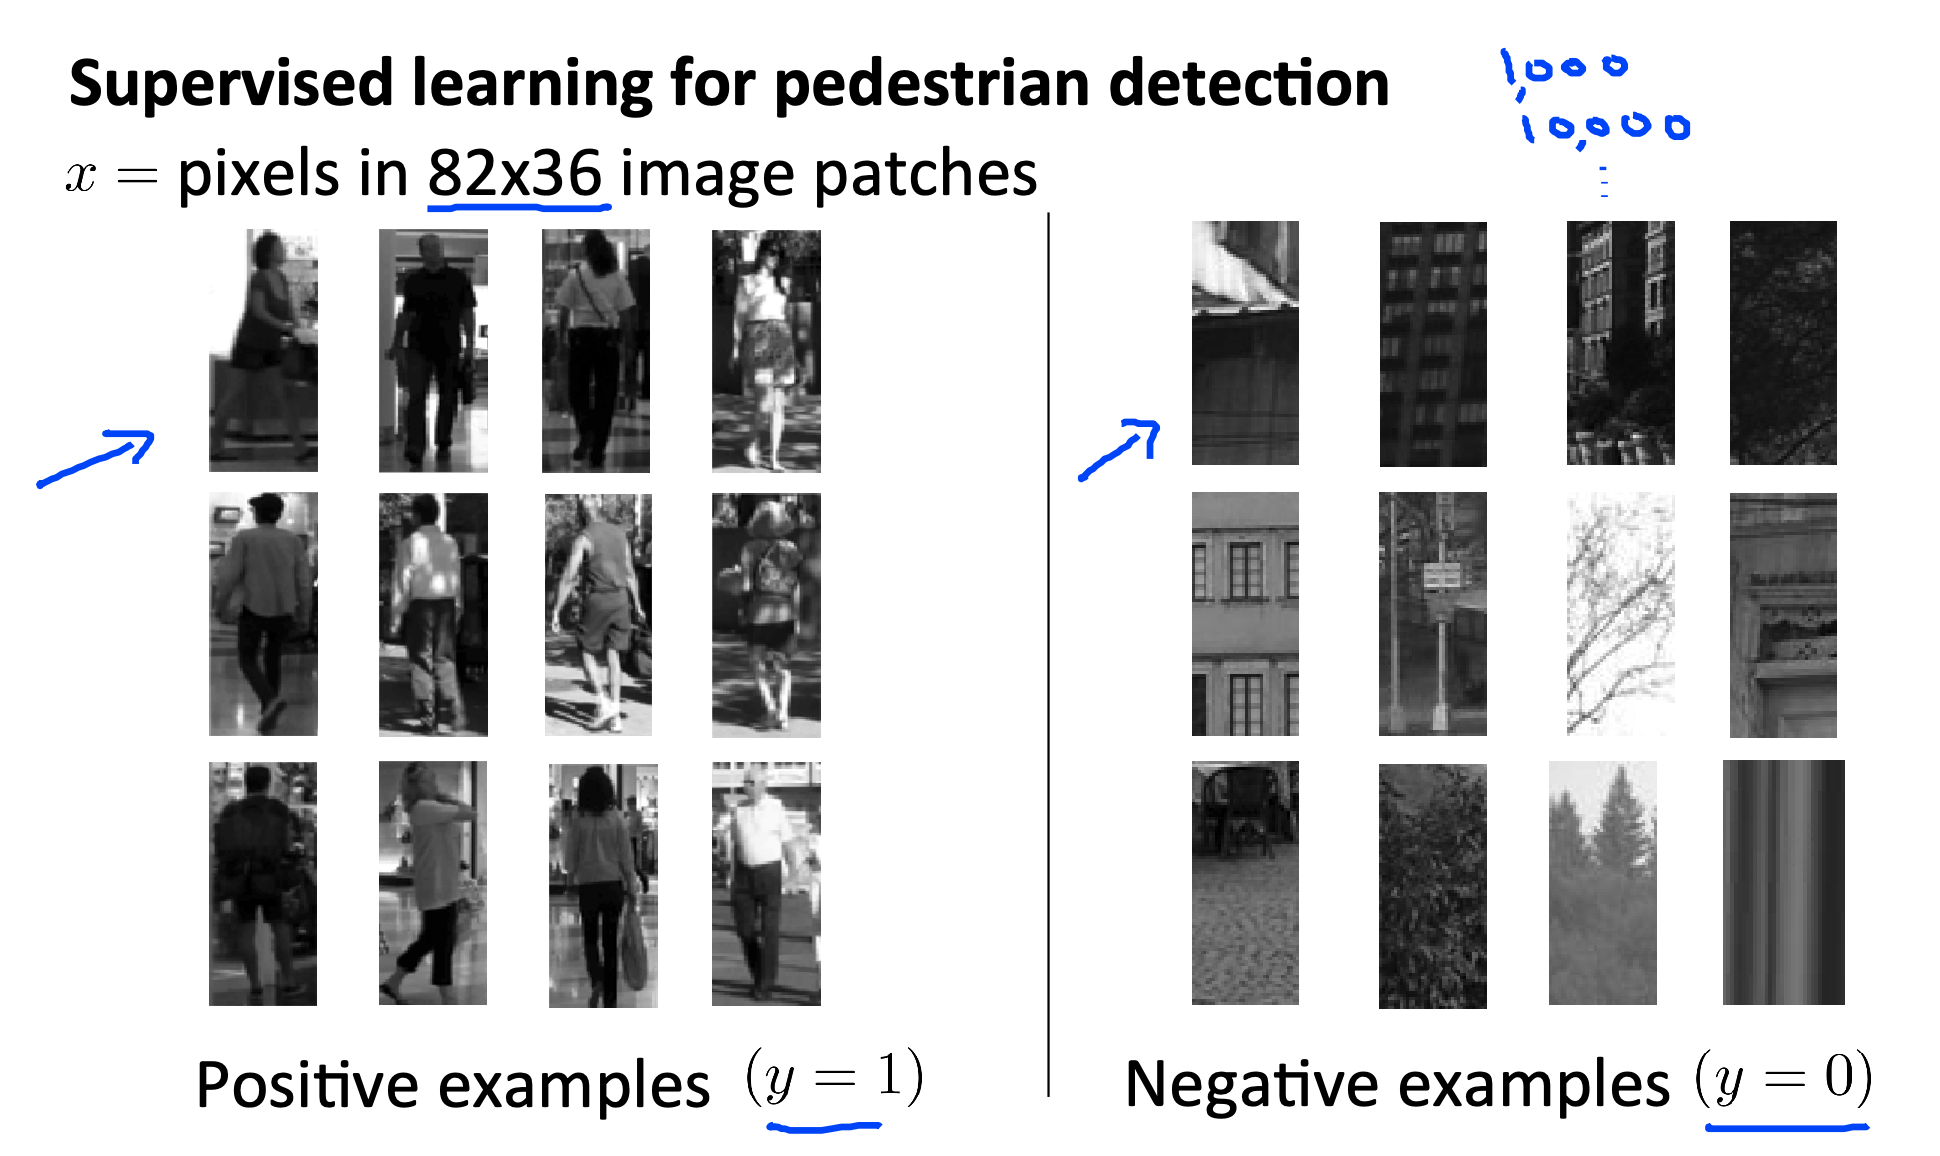
\includegraphics[width=0.8\textwidth]{image/pedestrian-example.png}
        \caption{Supervised learning for pedestrian detection: examples}
        \label{fig:pedestrian-example}
    \end{figure}

    \begin{itemize}
        \item Example: supply patches of either pedestrian (y=1)  and non-pedestrian (y=0). (Fig: \ref{fig:pedestrian-example})
        \item Sliding window detection: divide test image into multiple grids; the width of the grid (window) is called the step-size, or stride. 
        \item Slide the window along the test image. 
    \end{itemize}

    \subsubsection{Returning to text detection}
    \begin{figure}[htpb]
        \centering
        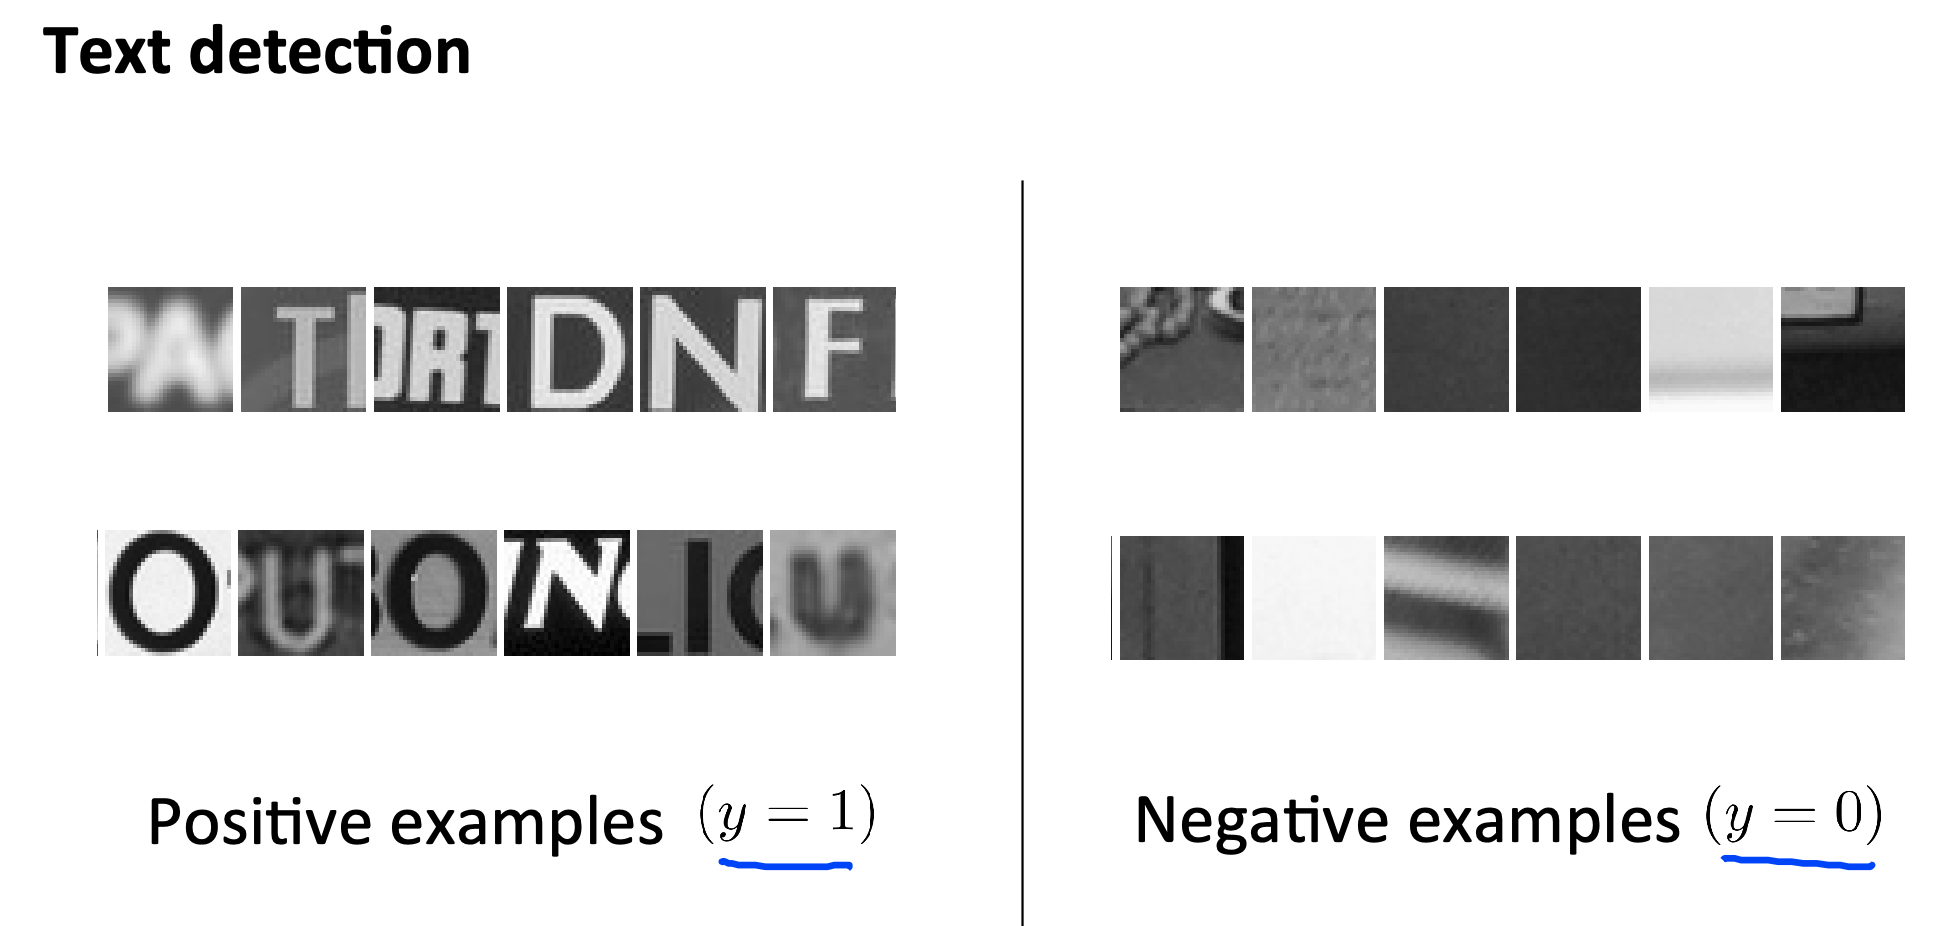
\includegraphics[width=0.8\textwidth]{image/text-detection-example.png}
        \caption{Supervised learning for text detection: examples}
        \label{fig:text-detection-example}
    \end{figure}


    \begin{itemize}
        \item Text detection is reflected as spectrum of white (highly probable text region) to black (low probability of text region). See Fig \ref{fig:text-detection}.

        \item Expansion: for every pixel: \emph{is it within x of a white pixel?}
        \item Filtering through aspect ratio: usually text boxes are wider than height. 
    \end{itemize}
    
    \begin{figure}[htpb]
        \centering
        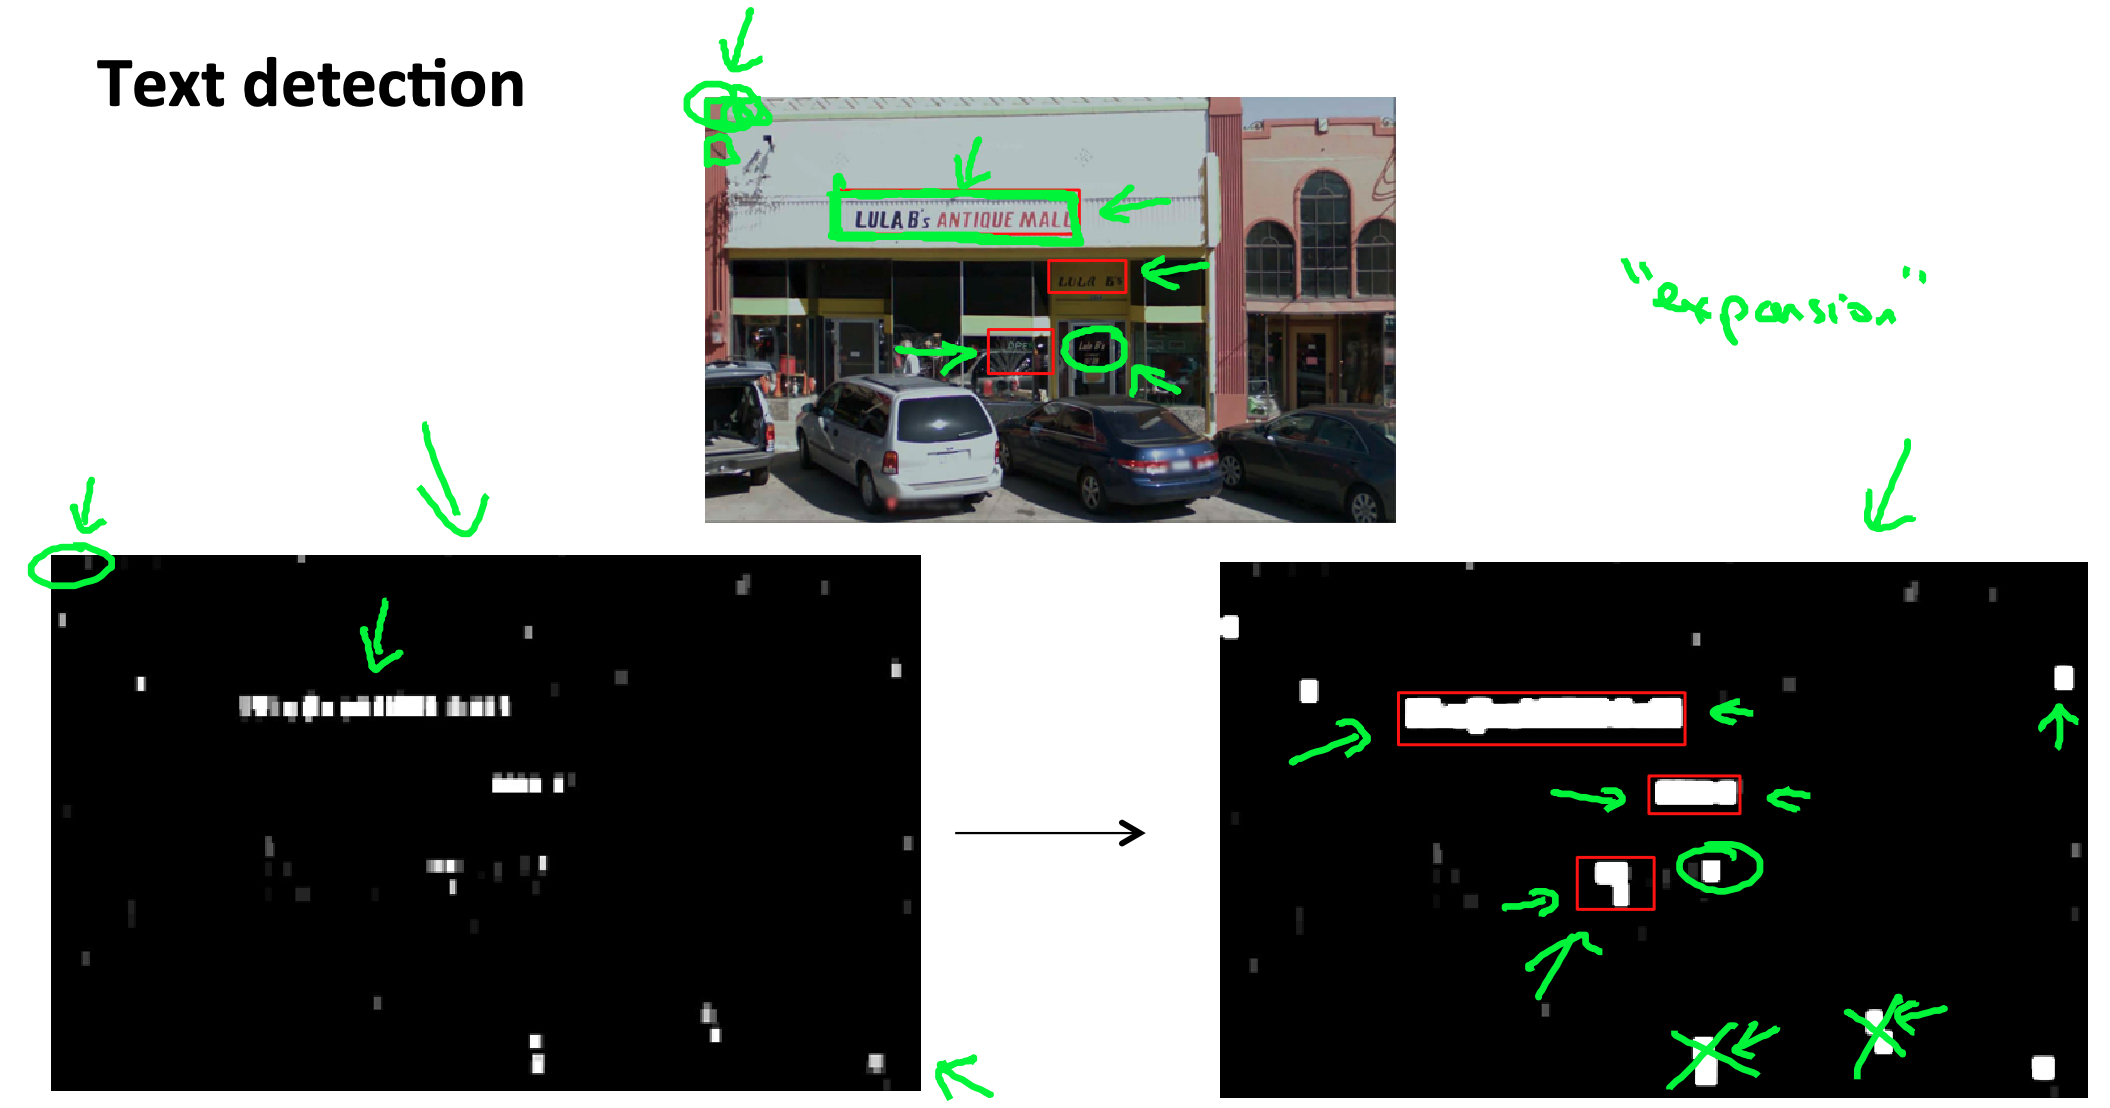
\includegraphics[width=0.8\textwidth]{image/text-detection.png}
        \caption{Text detection results}
        \label{fig:text-detection}
    \end{figure}

    Character segmentation: is there a split between two characters?
    \begin{figure}[htpb]
        \centering
        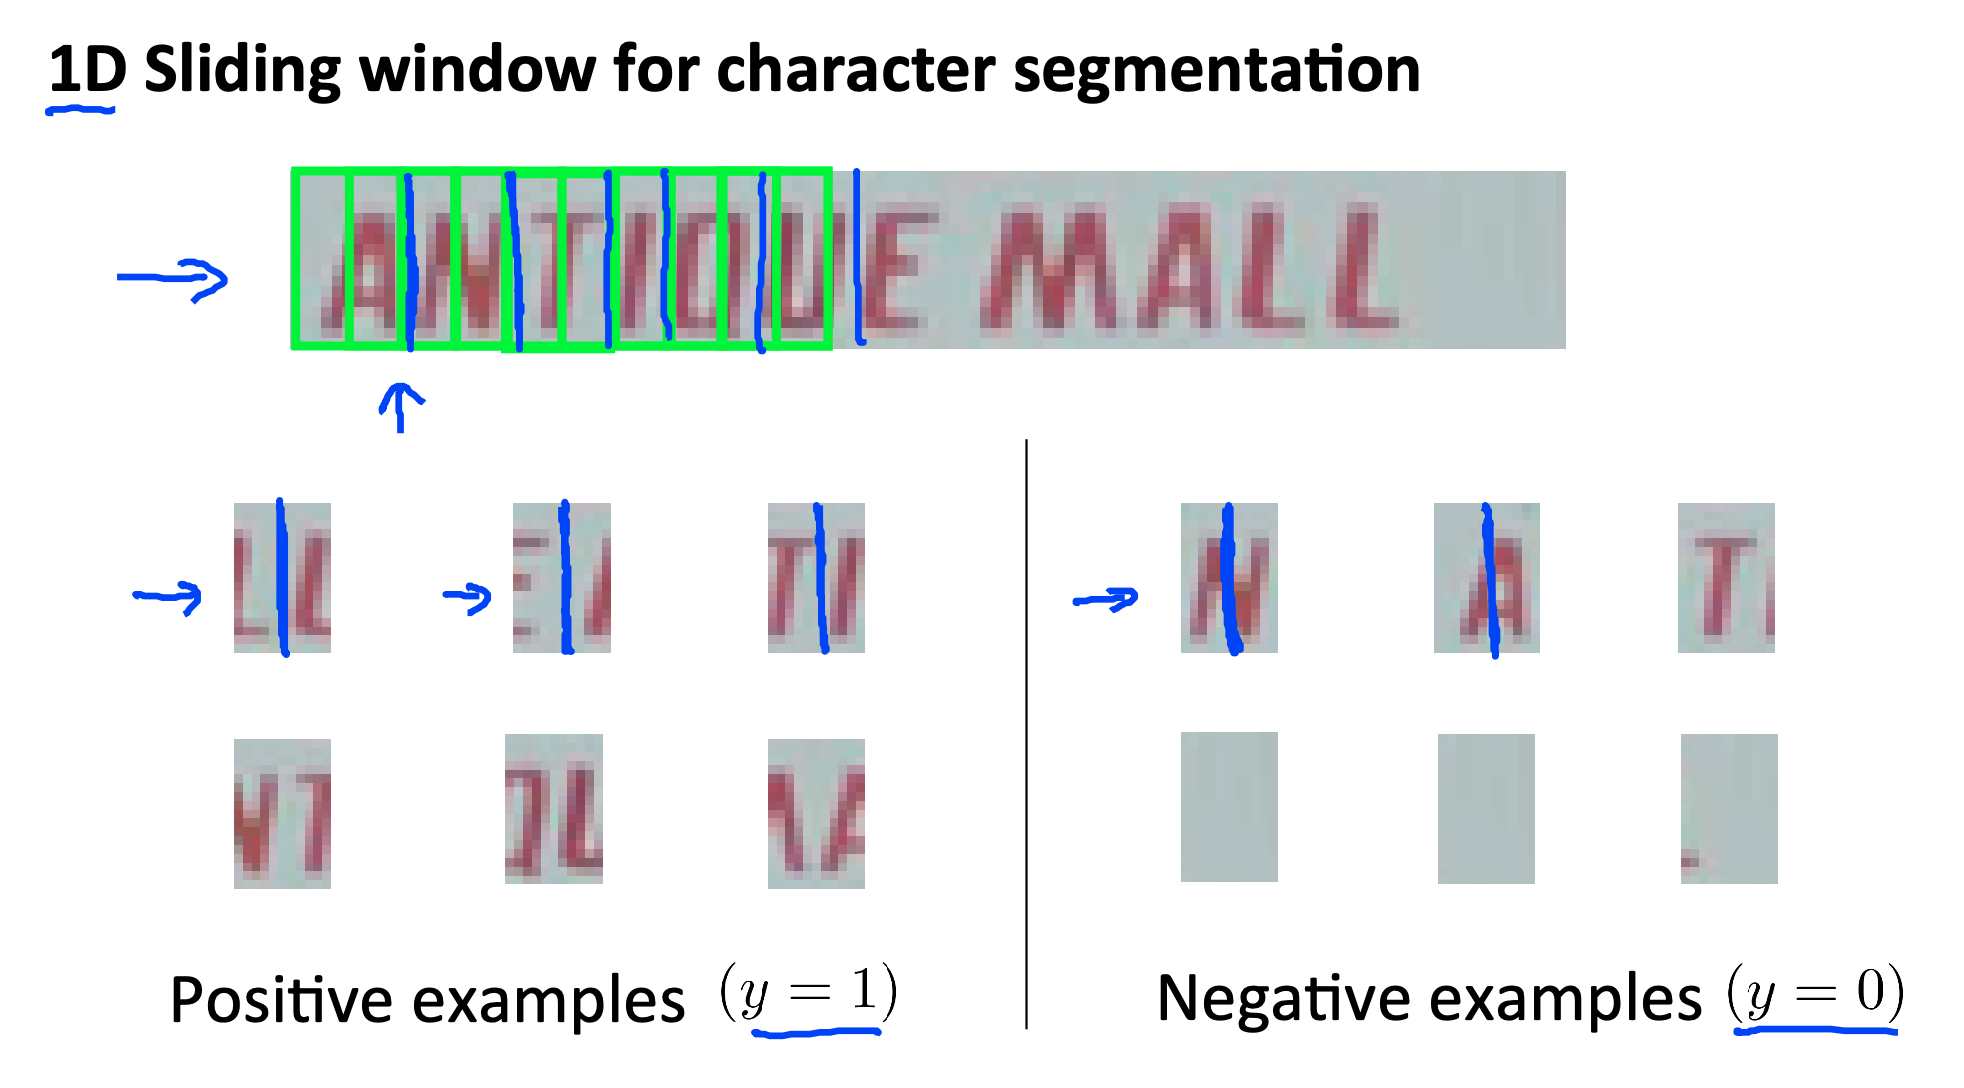
\includegraphics[width=0.8\textwidth]{image/character-segmentation.png}
        \caption{Character segmentation examples}
        \label{fig:character-segmentation}
    \end{figure}

\subsection{Getting lots of data: Artificial Data synthesis}
\begin{enumerate}
    \item Creating data from scratch: take computer-generated font and paste on random background image.
    \item Amplify a small training set: synthesizing data by introducing distortions; e.g. text distortion (Fig \ref{fig:text-detection-distortion} ), audio distortion for speech recognition.  
\end{enumerate}
    \begin{figure}[htpb]
        \centering
        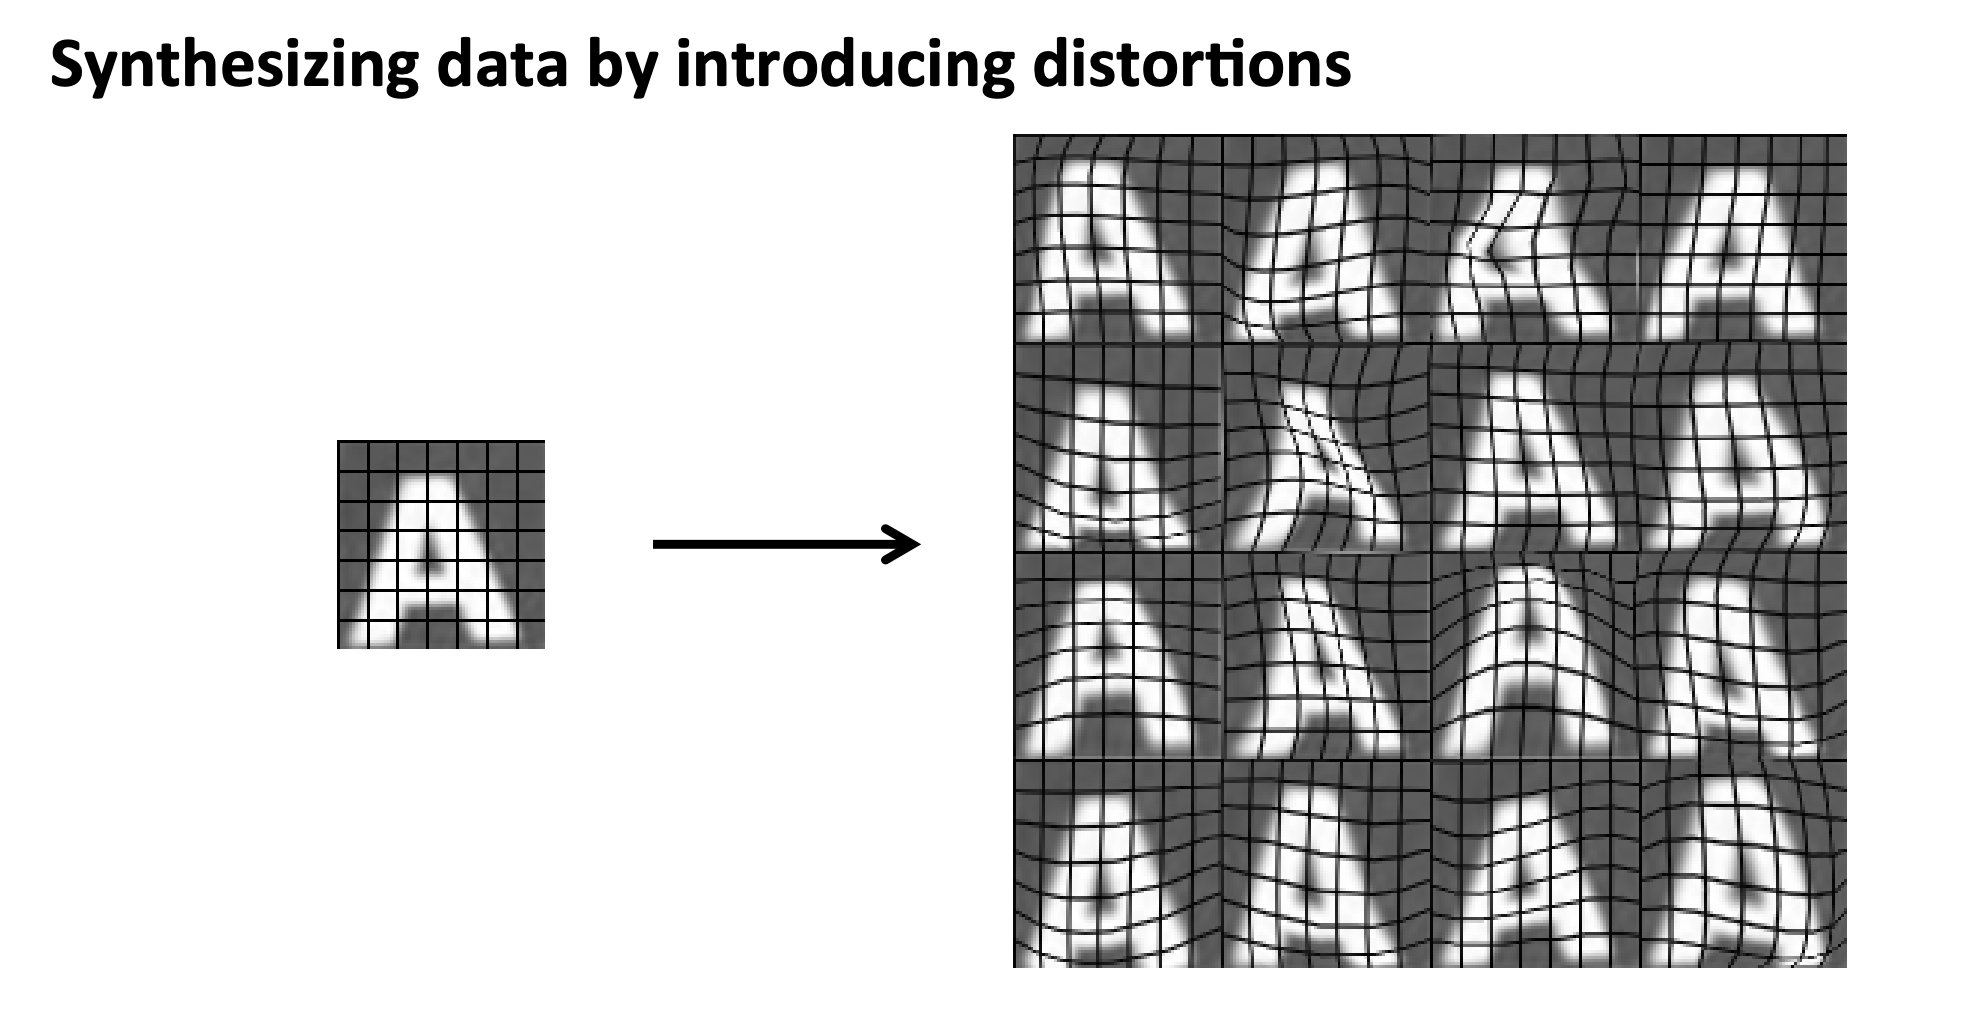
\includegraphics[width=0.8\textwidth]{image/text-detection-distortion.png}
        \caption{Introducing distortion to amplify dataset}
        \label{fig:text-detection-distortion}
    \end{figure}



\begin{enumerate}
    \item Distortion introduced should be representation of the type of noise/distortions in the test set. Usually does not help to add purely random/ meaningless noise to your data. 
    \item Make sure you have low bias classifier before expending the effort. (Plot learning curves). E.g. keep increasing the number of features/number of hidden units in neural network until you have a low bias classifier. 
    \item How much work would it be to get 10x as much data as we currently have? 
            \begin{itemize}
                \item Artificial data synthesis.
                \item Collect/label it yourself.
                \item Crowd source: e.g. Amazon Mechanical Turk
            \end{itemize}
\end{enumerate}


\subsection{Ceiling analysis: what part of the pipeline to work on next}
    \textbf{Ceiling analysis}: estimate the errors due to each component.
\begin{itemize}
    \item Simulate (through manual work) the accuracy of each component if the previous pipeline stage had given 100\% accurate data. Manual work to just supply the expected correct output. 
    \item This analysis is incremental, we incrementally cut down the pilpeline starting from the first stage. As such, it is expected at the last stage (giving correct output of last stage), measured overall system accuracy should be 100\%.
    \item Need to measure the delta.

        \begin{figure}[htpb]
            \centering
            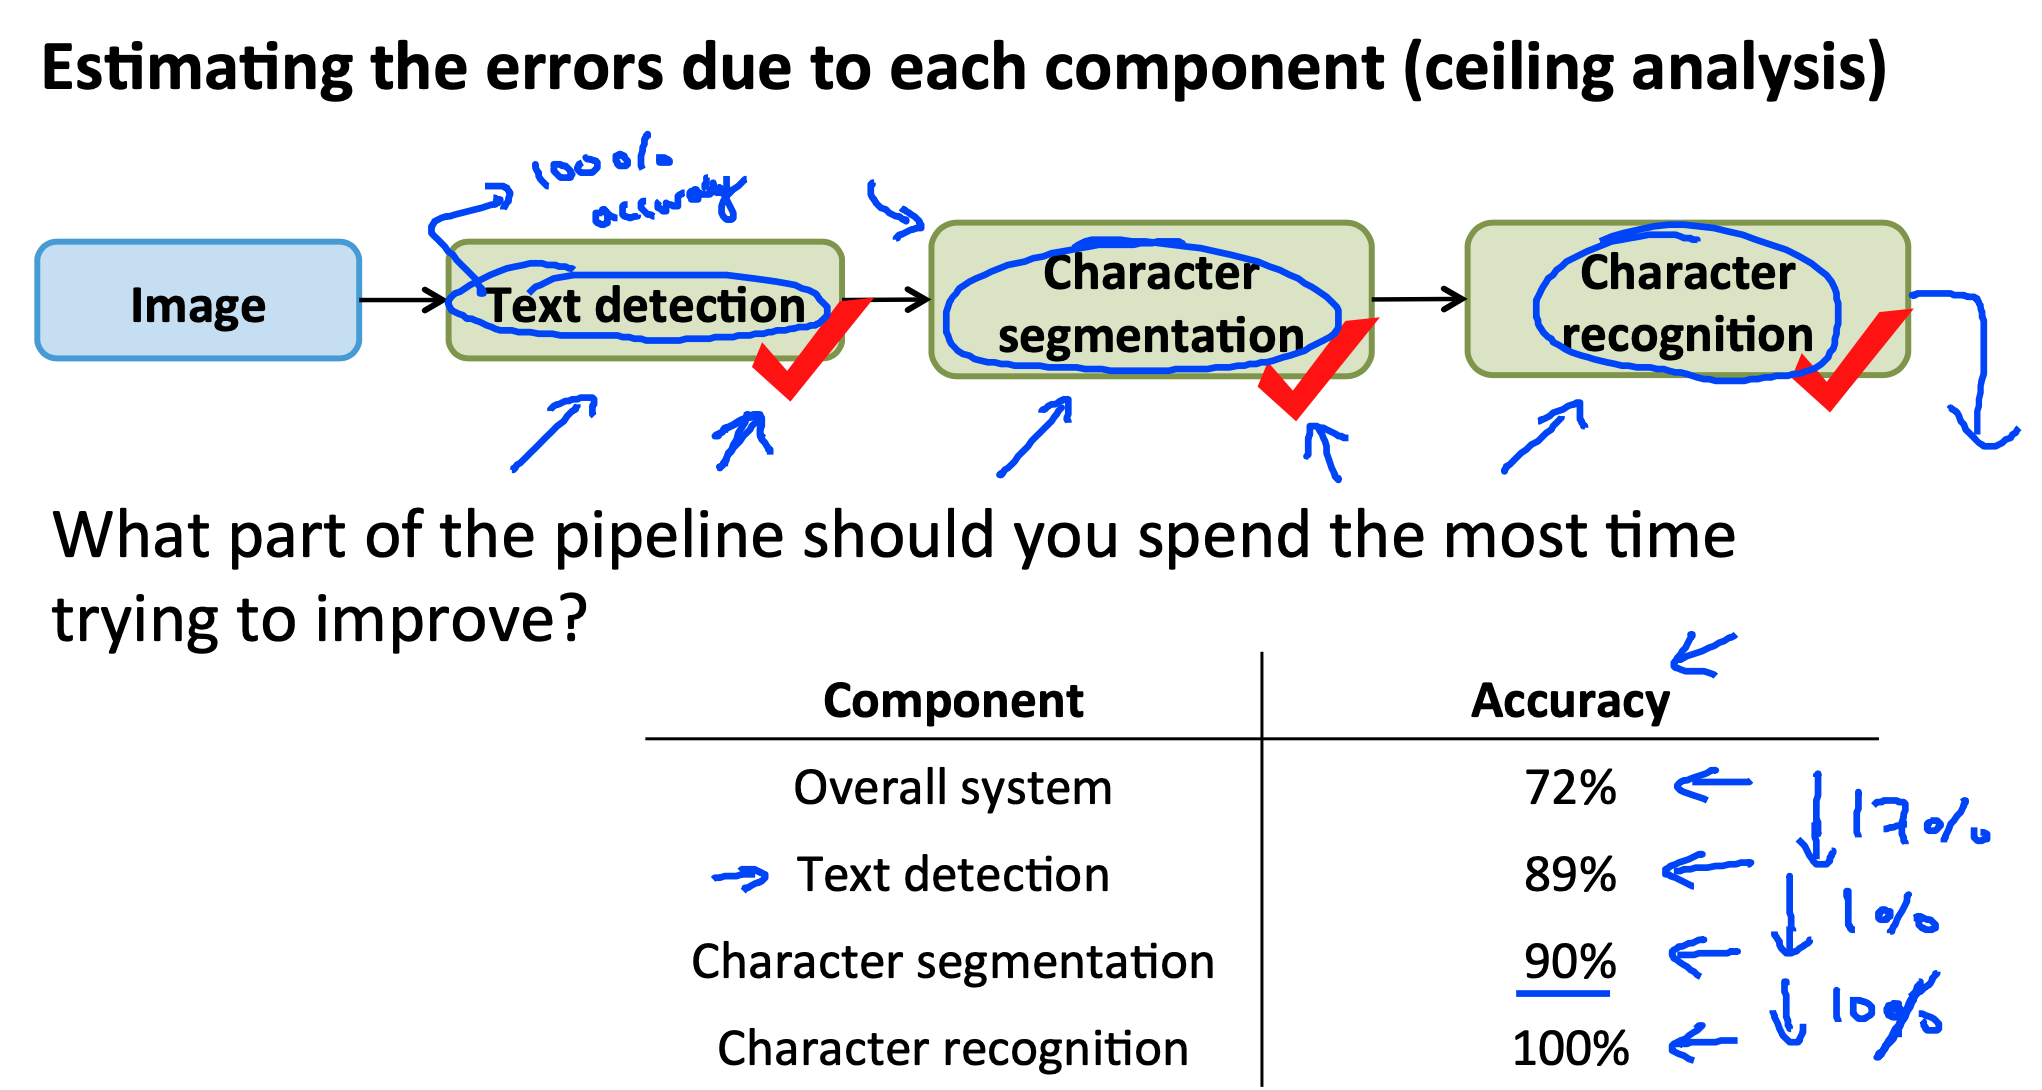
\includegraphics[width=0.8\textwidth]{image/ceiling-analysis.png}
            \caption{Ceiling analysis OCR}
            \label{fig:ceiling-analysis}
        \end{figure}
\end{itemize}
